\title{Lecture 2: Generative Models - Monte Carlo Tree Search}
% \author{Qi Zhang}
% \date{Last Updated: September 2025}

\section{Online Planning with a Generative Model}
Planning algorithms like value iteration (VI) and policy iteration (PI) solve Bellman (optimality) equations with the full knowledge of the MDP (e.g., the exact distribution over next states given any state-action pair).
We here consider a more relaxed setting, where transition and reward functions $(P, R)$ of the underlying (infinite-horizon) MDP $M=(\mathcal{S},\mathcal{A},P,R,\gamma)$ are unknown, but we can query them for any state-action pair to get samples, $s'\sim P(s,a), r\sim R(s,a)$, or $s',r\sim M(s,a)$ as a shorthand.
In this setting, we often say we have a {\em simulator} or a {\em generative model}.
In this note, we restrictively consider MDPs where every trajectory ends in a terminal state after a finite number of transitions so we can safely choose $\gamma=1$, examples including board games like chess and many others.

Moreover, VI and PI compute an optimal policy purely offline for all possible states and then look up the policy to select actions to take. While ensuring optimality, such {\em offline planning} methods are not feasible for large state spaces.
In this note, we are instead interested in the {\em online planning} paradigm where planning and action execution is interleaved: 
at the current state, a certain computation budget is allocated to try to figure out a good action to take; this process is repeated after taking that action and transiting to a next state.
This is much closer to how humans play games like chess.

\section{Monte Carlo Tree Search - The Algorithmic Template}
Monte Carlo Tree Search (MCTS) is a algorithmic technique to figure out a good action to take in current state by progressively building up a search tree where a parent-child connection represents a transition and nodes in the tree accumulates statistics from multiple sampled episodes.
More specifically, initializing the tree with the only node being the current state as the root, MCTS repeatedly performs the following procedures as depicted in Figure \ref{fig:mcts} and outlined in \ref{alg:mcts} and \ref{alg:mcts_procedures}:
\begin{enumerate}
    \item {Selection:} 
    From the root, navigate down the tree with transitions sampled from the generative model and some action-selection rule until a new transition occurs from a leaf node.
    \item {Expansion:}
    Create a new leaf by attaching that new transition to the tree.
    \item {Simulation:}
    Starting from the new leaf's state, simulate a trajectory by the generative model and some action-selection rule until reaching a terminal state.
    \item {Backpropagation:}
    Using the rewards from the root to the terminal state, modify the value estimates along the path.
\end{enumerate}
\begin{figure}[htb]
\centering
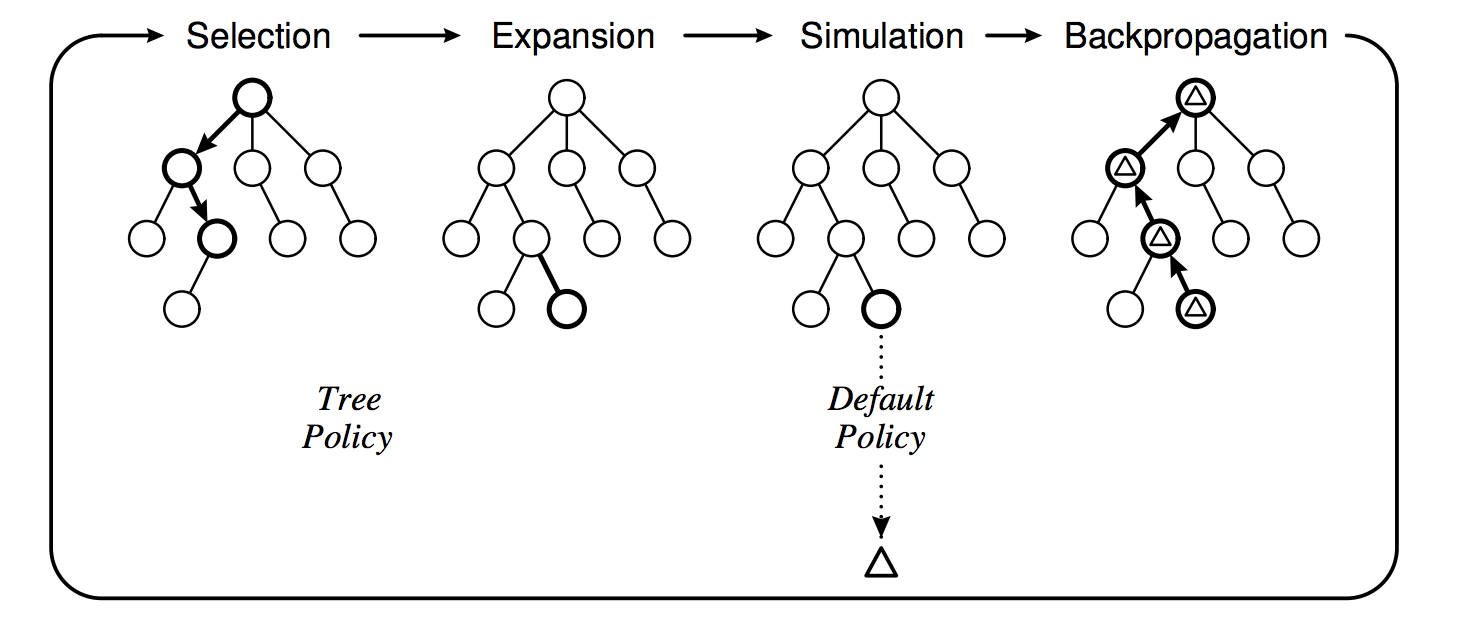
\includegraphics[width=0.9\textwidth]{lectures/figures/standard_mcts.png}
\caption{Illustration of an MCTS iteration (credit to \cite{mcts_survey}).}
\label{fig:mcts}
\end{figure}

Each node $\tau$ tracks $N_\tau$, the total number of sampled paths that visited this node's state, and $G^{\rm total}_\tau$ (i.e., $\tau.{\rm total\_reward}$ in Algorithms \ref{alg:mcts} and \ref{alg:mcts_procedures}), the total reward accumulated from that node to the terminal states over all $N$ paths. To select a good action from the root node, we hope the empirical mean of $G^{\rm total}_{\tau,a}/N_{\tau,a}$ well approximates Q-value of a reasonably good policy, where $G^{\rm total}_{\tau,a}$ is the total reward for all children of the node connected by a branch for action $a$ (respectively for $N_{\tau,a}$).
In the typical case where the state space is too huge to be fully explored, Selection (line \ref{alg:mcts_procedures:line:SelectAction} in Algorithm \ref{alg:mcts_procedures}) should strike a balance between exploration of unknown paths and exploitation of historically promising paths.
Expansion grows the tree, often by one leaf per iteration. We hope that each node on average gets a good number of sampled episodes to accumulate its statistics, so it is important not to grow the tree too fast.
Selection and Expansion together are sometimes referred to as Tree Policy.
Simulation aims to choose actions quickly, usually by some heuristics or just random action selection.
Various algorithmic choices for these procedures give rise to specific instantiations.
Section \ref{sec:UCT} discusses a well-known instantiation of this template, UCT.

\subsection*{Implementation details}
As above, the algorithmic description of MCTS is often based on the data structure of {\em state node}: a node is associated with a state $s$ along paths in the tree that visit this node, with its children indexed by $(a,s')$ for a transition of $(s,a,s')$.
In hw2.ipynb of our Homework 2, we adopt an alterative implementation that explicitly distinguishes between the state node, referred to as the {\em V-node}, and the action node that is referred to as the {\em Q-node}.
In a path, V-nodes are still associated with the states therein, while Q-node are associated with the actions.
Therefore, 
\begin{itemize}
    \item The two types of nodes are interleaved depth-wise: a V-node has only Q-nodes (but not V-nodes) as its children and a Q-node has only V-nodes (but not Q-nodes) as its children;
    \item The root node is always a V-node of current state. 
    \item The expansion happens upon an unseen transition $(s,a,s')$ starting from a leaf V-node of state $s$ and grows the tree with a new leaf V-node of state $s'$ and a new Q-node of action $a$ as its parent if $a$ has not been tried, so the leafs are always V-nodes. 
    \item Statistics such as $N_{\tau,a}$, $G^{\rm total}_{\tau,a}$, and step reward are accumulated at the corresponding Q-nodes, and V-node can thus access its statistics by aggregating its Q-node children. For example, $N_\tau=\sum_a N_{\tau,a}$ where $N_\tau$ is the number of visits for a V-node $\tau$, which equals to the summation over its Q-node children.
\end{itemize}


\begin{algorithm}
\caption{Monte Carlo Tree Search} \label{alg:mcts}
\begin{algorithmic}[1]
\Procedure{MonteCarloTreeSearch}{$\tau_0$}
  \Comment{Root node $\tau_0$}
  % \State $\tau_0$ = \textsc{InitNode}($s_0$)
  \Repeat
    \State $\tau$ $\gets$ \textsc{TreePolicy}($\tau_0$) \Comment{New leaf $\tau$, total reward $G_i$ cumulated from root $\tau_0$}
    \State $s$ $\gets$ $\tau$.state
  	\State $G$ $\gets$ \textsc{DefaultPolicy}($s$) \Comment{$G$ is total reward cumulated from state $s$}
    \State \textsc{Backup}($\tau$, $G$) \Comment{Update node statistics along the path}
  \Until{\textsc{Timeout}()}
  \State \Return \textsc{BestAction}($\tau_0$) \Comment{Pick the approximately optimal root-level action}
\EndProcedure\\

\Procedure{InitNode}{$s$}
\State $\tau.{\rm parent}\gets {\rm null}$
  \State $\tau.{\rm state}\gets s$
  \State $\tau.{\rm count}\gets 0$
  \State $\tau.{\rm total\_reward}\gets 0$ \Comment{Cumulated over timesteps and episodes}
  \State $\tau.{\rm children}[a][s']\gets {\rm null}$, for all $a, s'$
  \State \Return $\tau$
\EndProcedure

\end{algorithmic}
\end{algorithm}

\begin{algorithm}
\caption{Monte Carlo Tree Search - Procedures} \label{alg:mcts_procedures}
\begin{algorithmic}[1]
\Procedure{TreePolicy}{$\tau_0$}
  \State $\tau, s  \gets$ $\tau_0$, $\tau_0$.state
  \While{\textsc{Nonterminal}($s$)}
  	\State $a \gets$ \textsc{SelectAction}($\tau$) \Comment{Heuristically select an action} \label{alg:mcts_procedures:line:SelectAction}
    \State $s',r \sim M(s,a)$  \Comment{Sample next state and reward from generative model}
    \If{$\tau\textrm{.children}[a][s'] =$ null} \Comment{Is this the first observation of $s \xrightarrow{a} s'$?}
    	\State $\tau' \gets$\textsc{InitNode}($s'$) \Comment{Initialize leaf node for state $s'$}
        \State $\tau'.{\rm parent } \gets \tau\textrm{.children}[a][s']$ \Comment{Attach leaf node to the tree}
        \State $\tau\textrm{.children}[a].{\rm reward} \gets r$      \Comment{Record $r=R(s,a)$}
        \State \Return $\tau\textrm{.children}[a][s']$ \Comment{Move on to simulation phase}
    \EndIf
    \State $\tau\textrm{.children}[a].{\rm reward} \gets r$      \Comment{Record $r=R(s,a)$}
    \State $\tau \gets \tau\textrm{.children}[a][s']$
    \State $s \gets s'$
  \EndWhile
  \State \Return $\tau$
\EndProcedure\\

\Procedure{DefaultPolicy}{$s$} \Comment{Decision policy for simulation}
 \State $G=0$
  \While{\textsc{Nonterminal}($s$)}
  	\State $a \sim$ \textsc{DefaultActionSelection}($s$) \Comment{e.g., randomly select an action from $\mathcal{A}$}
  	\State $s',r \sim M(s,a)$  \Comment{Sample next state and reward from generative model}
    \State $G \gets G + r$
  \EndWhile
  \State \Return $G$
\EndProcedure\\

\Procedure{Backup}{$\tau, G$} \Comment{$G$ is the total reward cumulated from node $\tau$}
  \Repeat
  	\State $\tau\textrm{.total\_reward} \gets \tau\textrm{.total\_reward} + G$
  	\State $\tau\textrm{.count} \gets \tau\textrm{.count} + 1$
  	\State $\tau, a \gets \tau\textrm{.parent}$ \Comment{$a$ is the action connecting the two nodes}
    \If{$\tau$ is not null}
        \State $G\gets G + \tau.{\rm children}[a].{\rm reward}$ \Comment{Add step reward along the path}  
    \EndIf 
  \Until{$\tau$ is {null}}
  \State \Return
\EndProcedure\\

\Procedure{BestAction}{$\tau$} \Comment{Pick the empirically best action at node $\tau$}
  \State \Return $\argmax_{a \in \mathcal{A}} \frac{\sum_{\tau' \in \tau\textrm{.children}[a][\cdot]} \tau'\textrm{.total\_reward}}{\sum_{\tau' \in \tau\textrm{.children}[a][\cdot]} \tau'\textrm{.count}}$
\EndProcedure
\end{algorithmic}
\end{algorithm}

\newpage\clearpage
\section{UCT}
\label{sec:UCT}
UCT \cite{uct}, Upper Confidence Bounds (UCB) applied to Trees, applies the UCB algorithm \cite{ucb} to the Selection procedure of MCTS to balance the exploration-exploitation tradeoff.
Specifically, UCT's Selection selects the action at each (V-)node $\tau$ (line \ref{alg:mcts_procedures:line:SelectAction} in Algorithm \ref{alg:mcts_procedures}) that maximizes the upper confidence bound on the estimated total reward from that node:
\begin{align*}
    \argmax_{a\in\mathcal{A}} \quad {\rm UCB}(\tau,a):= \frac{G^{\rm total}_{\tau,a}}{N_{\tau,a}} + c\sqrt{\frac{\ln(N_s)}{N_{\tau,a}}}
\end{align*}
where $c>0$ is a hyperparameter controlling how much exploration is favored over exploitation. 

% \section{AlphaGo Zero}
% \label{sec:AlphaGo Zero}


% \newpage\clearpage
\bibliographystyle{unsrt}
\bibliography{references}